\usetikzlibrary{arrows.meta,calc,decorations.pathreplacing,fit}

\tikzset{
    simple wire/.style={very thick,>=Latex},
    wire/.style={line width=1.5pt,>=Latex},
    wire small/.style={line width=1pt,>=Latex},
    binLabel/.style={font=\tt},
    hiBox/.style={red, very thick, draw},
    >=Latex,
}
\begin{frame}[fragile,label=moveBits]{moving bits in hardware (one way)}
    % FIXME: diagram: wire bundle splitting getting opcode
    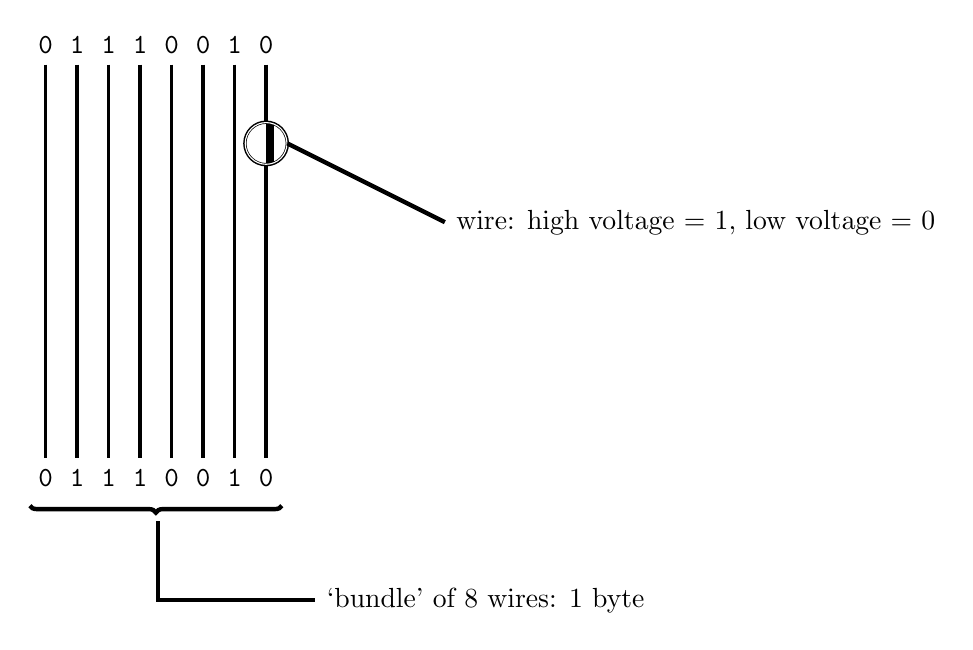
\begin{tikzpicture}
\foreach \x/\v in {0/0,0.4/1,0.8/1,1.2/1,1.6/0,2.0/0,2.4/1,2.8/0} {
    \draw[simple wire] (\x, 0) node[above] {\tt\v} -- (\x, -5) node[below] {\tt\v};
};
        \draw[fill=white,very thick] (2.8, -1) circle (.27cm);
        \draw[line width=3pt] (2.85, -1) -- ++ (0, -.27);
        \draw[line width=3pt] (2.85, -1) -- ++ (0, .27);
        \draw[white] (2.8, -1) circle (.265cm);
        \draw[ultra thick] ($(2.8, -1) + (0.27, 0)$) -- ++(2cm, -1cm)
            node[right] {
                wire: high voltage = 1, low voltage = 0
            };
        \draw[decorate,decoration={brace,mirror},ultra thick] (-.2, -5.6) -- ++(3.2, 0);
        \draw[ultra thick] (1.425, -5.8) |- ++(2cm, -1cm) node[right] {`bundle' of 8 wires: 1 byte};
\end{tikzpicture}
\end{frame}
